\documentclass[12pt]{report}
\usepackage[print,nopanel]{pdfscreen}
%\begin{print}
\usepackage{lipsum}% http://ctan.org/pkg/lipsum
\usepackage{titletoc}% http://ctan.org/pkg/titletoc
%\section{type}
\usepackage{lastpage}
\usepackage{macro/macro}
\usepackage{float}
\usepackage{wrapfig}
\usepackage{fancyhdr}
\usepackage{verbatim}
\usepackage[Glenn]{fncychap}
\usepackage{times}
\lhead{\large\bfseries LibreCAD v3 Development}
\usepackage[left=3.5cm, right=1.5cm, top=2.5cm, bottom=1.5cm]{geometry}
\pagestyle{fancy}
%\end{print}
\begin{screen}

\usepackage{setspace}
\linespread{1.5}
\renewcommand{\rmdefault}{ptm}
\end{screen}
\screensize{8cm}{9cm}
\overlay{overlay8.pdf}
\usepackage{graphicx}

\begin{document}
\thispagestyle{empty}
\begin{center}
{\fontsize{24}{30}\selectfont Project Report}

\vspace*{\baselineskip}

{\fontsize{18}{30}\selectfont on}

\vspace*{\baselineskip}

{\bfseries\fontsize{24}{30}\selectfont ``LibreCAD v3''}

\vspace*{2\baselineskip}

{
    \fontsize{10}{30}\textit {SUBMITTED IN PARTIAL FULLFILLMENT OF THE REQUIREMENTS}
    
    \vspace*{\baselineskip}
    
    \textit{ FOR THE AWARD OF DEGREE}
}

\vspace*{2\baselineskip}

{\bfseries\fontsize{16}{30}\selectfont ``\textit{Bachelors of Technology}''}

\vspace*{\baselineskip}

In

\vspace*{\baselineskip}

{\bfseries\fontsize{14}{20}\selectfont Computer Science and Engineering }
\vspace*{\baselineskip}

To
\vspace*{\baselineskip}

{\bfseries\fontsize{14}{20}\selectfont Punjab Technical University, Jalandhar.}

\vspace*{3\baselineskip}

{\bfseries\fontsize{12}{20}\selectfont SUBMITTED BY}

{\fontsize{12}{20}\selectfont

GAGANJYOT SINGH

CSE

Semester V

1306677

2012 - 2016

}

\vspace*{2\baselineskip}


\includegraphics[scale=1.5]{images/CEC.jpg}

\vspace*{2\baselineskip}

\begin{flushbottom}

{\bfseries\fontsize{14}{30}\selectfont DEPARTMENT OF COMPUTER SCIENCE AND ENGINEERING}

\vspace*{\baselineskip}
{\bfseries\fontsize{14}{30}\selectfont Chandigarh Enginnering College, Landran}

\vspace*{\baselineskip}
{\fontsize{14}{30}\selectfont Mohali, Punjab  - 140307}

\end{flushbottom}
\end{center}

\begin{screen}
\ppttitle
\end{screen}
\footskip 0.7cm
\thispagestyle{empty} 
\newpage
\pagenumbering{Roman}
\cfoot{\thepage}

\begin{center}
\huge{Acknowledgement}
\end{center}
Foremost of all, I express my sincere indebtedness to the “Almighty”, for bestowing me with all the favourable circumstances and kept me in high spirits, I would like to whole heartedly thank Dr. H.S. Rai Dean, Testing and Consultancy Cell, Guru Nanak Dev Engineering College, Ludhiana who is a vast sea of knowledge and without whose constant and never ending support and motivation, it would never have been possible to complete the project and other assignments so efficiently and effectively.\\\\
I would like to thank Christopher Sean Morrison ( Project Leader BRL-CAD ) to consider LibreCAD under its organisation. Ries Van Twisk and Dongxu Li ( Core Developers of LibreCAD and my Mentors during the Google Summer of Code Programme ) for having firm faith in me and constantly encouraging and helping out through out the development of the project.\\\\
Extending the thanks, I thank the Google Inc. for giving me opportunity to work under an opensource project for 3 months under the Google Summer of Code 2014.\\\\
Last but not the least, I am very great full to my professor, Mr. Rajeev Sharma for his patience, encouragement, and many fruitful discussions. I would like to thank , Head of Department of Computer Science and Engineering, Chandigarh Engineering College, Landran. I wish to express my appreciation to my family for my continuous love and encouragement, for always believing in me, for never failing to provide all the support, and for coping with the pressure that naturally comes with such endeavour.\\\\

\newpage

\begin{Large}
\begin{center}Abstract\end{center}
\end{Large}

\noindent LibreCAD v3 development project discusses the work done in computer-aided-design. Computer-aided design (CAD) is the use of computer systems to assist in the creation, modification, analysis, or optimization of a design in engineering sciences. I explored  LibreCAD  Source  Code. LibreCAD is Free and Open Source  2D  CAD   application  that  you  can  download  and  install  for  free.  There  is  a  large base  of  satisfied  LibreCAD   users  worldwide,  and  it  is  available  in  more  than  20  languages  and  for  all major  operating  systems,  including  Microsoft  Windows,  Mac  OS  X  and  Linux .  Librecad  is  an  application  for  computer  aided  design  in  two dimensions  .  With  librecad   you   can  create  technical  drawings  such  as  plans  for  buildings,  interiors, mechanical parts or schematics and diagrams. Basically, LibreCAD is used to make 2D design. \\

\noindent LibreCAD was forked from QCAD Software 12 years ago. Since then technologies changed a lot and LibreCAD was on a Quite old code base. We have designed a new version of LibreCAD Code named as v3 updating the LibreCAD to new technologies and the real world exposure enhancing the internals of LibreCAD to be able to handle Large files efficiently and a MVC like modular approach so as to make v3 capable of integration into other softwares ( BRL-CAD being a live example of the use case except the LibreCAD itself).

\noindent Also, this project is completely open source and the entire code is available to the user as and when required. There is also Complete developer's Documentation as well as User manual alongwith it that helps using it a lot easier.


\newpage
\tableofcontents
\newpage
\listoffigures
\newpage

\pagenumbering{arabic}
\cfoot{\thepage}

\newpage
\chapter{Introduction To Organisation}
\input{input/company.tex}
\newpage
\chapter{Introduction To Project}
\input{input/project-preview.tex}
\input{input/librecad.tex}
\chapter{Project Work}
\newpage
\section{LibreCAD v3 Kernel Development}
This is the CAD Kernel I have devloped during my 6 week training project. Iwas hired by Google for 3 months and paid a stipend of Rs. 300000 during the work. This CAD kernel is developed for the opensource CAD organisation LibreCAD under the supervision of BRL-CAD. 
\begin{figure}[h]
\begin{center}
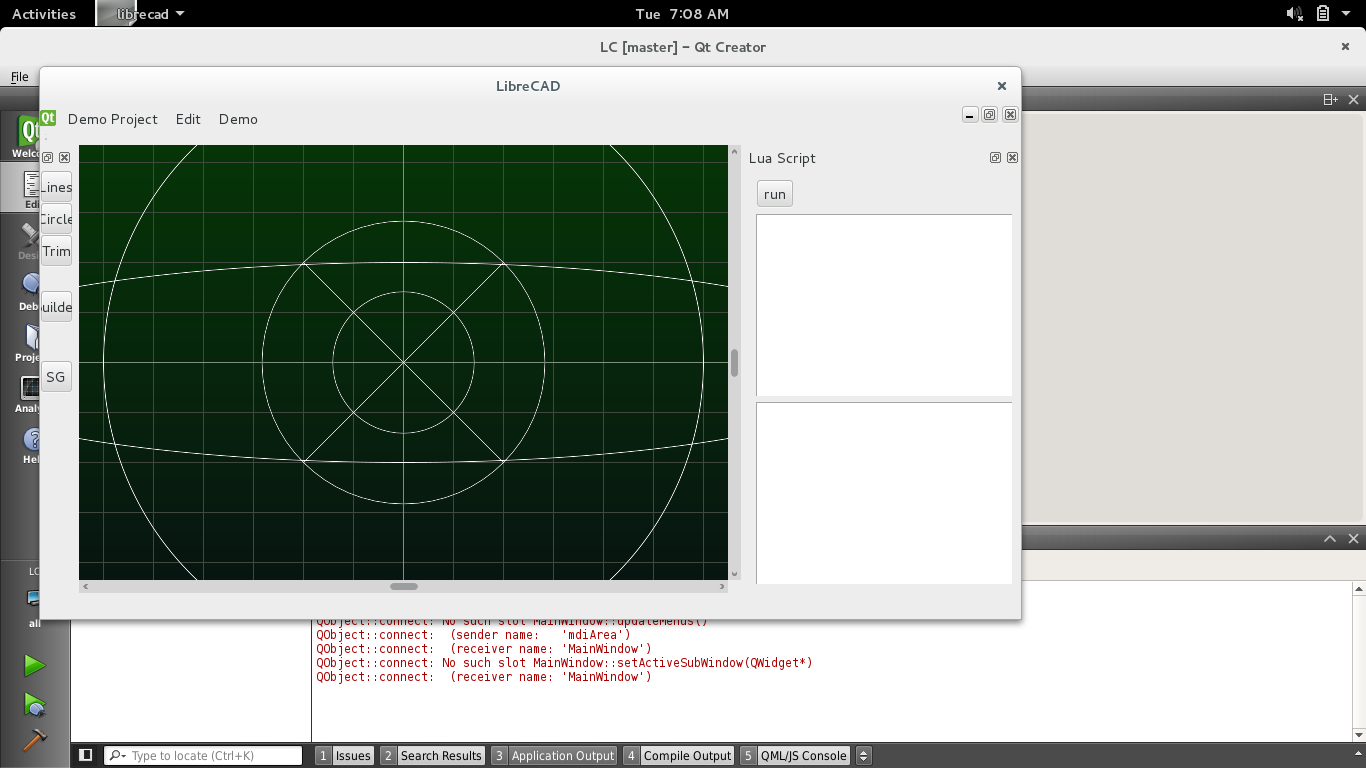
\includegraphics[scale=0.3]{images/cad/simplerun.png}
\caption{v3- The advanced 2D kernel}
\end{center}
\end{figure}

It has the following features:
\begin{itemize}
\item New
\item Undo
\item Redo
\item Add Random Circle
\item Add Random Arc
\item Add Random Lines
\item Clear Undo Stack
\end{itemize}

The idea of LibreCAD v3 Kernel Development was to build a stable kernel for the improvement of CAD and Opensource CAD. LibreCAD 3 has been divided into 3 modules.

\begin{itemize}
\item Kernel
\item Viewer
\item UI
\end{itemize}

Though the code is still in development, variations may apply. There is an additional module for scripting. Users can develop their on modules in their preferred langauge may it be python, lua, ruby.
We preferred lua since it was lightweight and simple.
The UI part of LibreCADv3 is to be rewritten hence it is disabled at the moment. Figures can be drawn using the lua script coding.

\begin{figure}[h]
\begin{center}
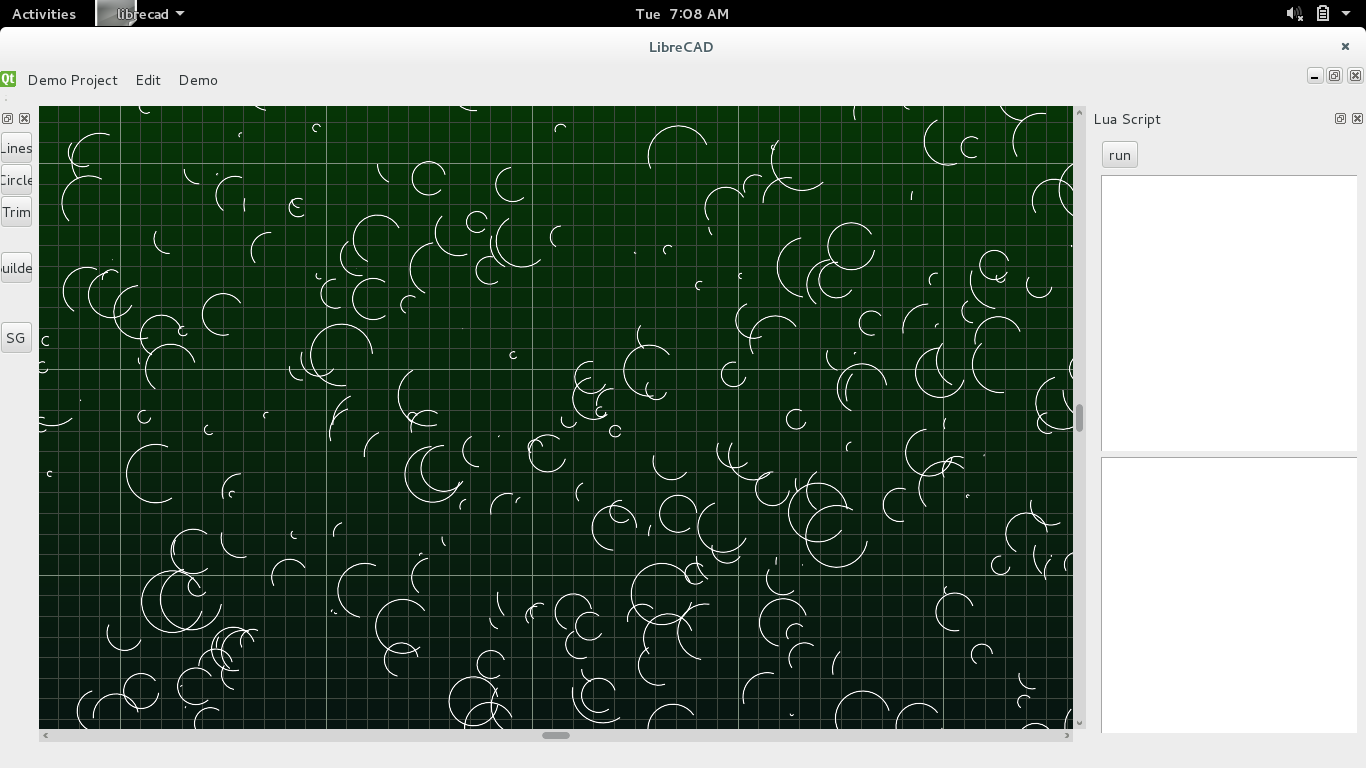
\includegraphics[scale=0.3]{images/cad/randomarc.png}
\caption{ Random arcs generated while testing. }
\end{center}
\end{figure}
\begin{figure}[h]
\begin{center}
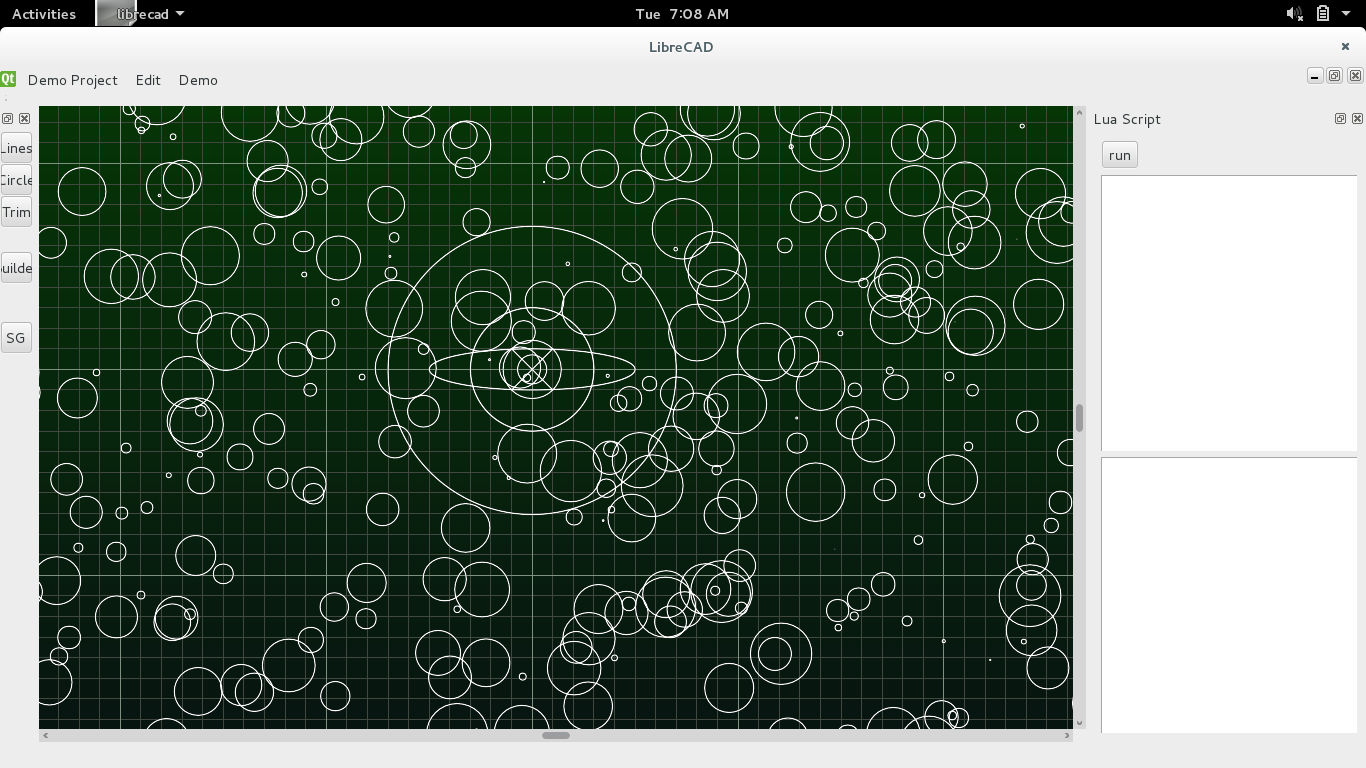
\includegraphics[scale=0.3]{images/cad/randomcircle.png}
\caption{ Random Circles generated during testing. }
\end{center}
\end{figure}
\begin{figure}[h]
\begin{center}
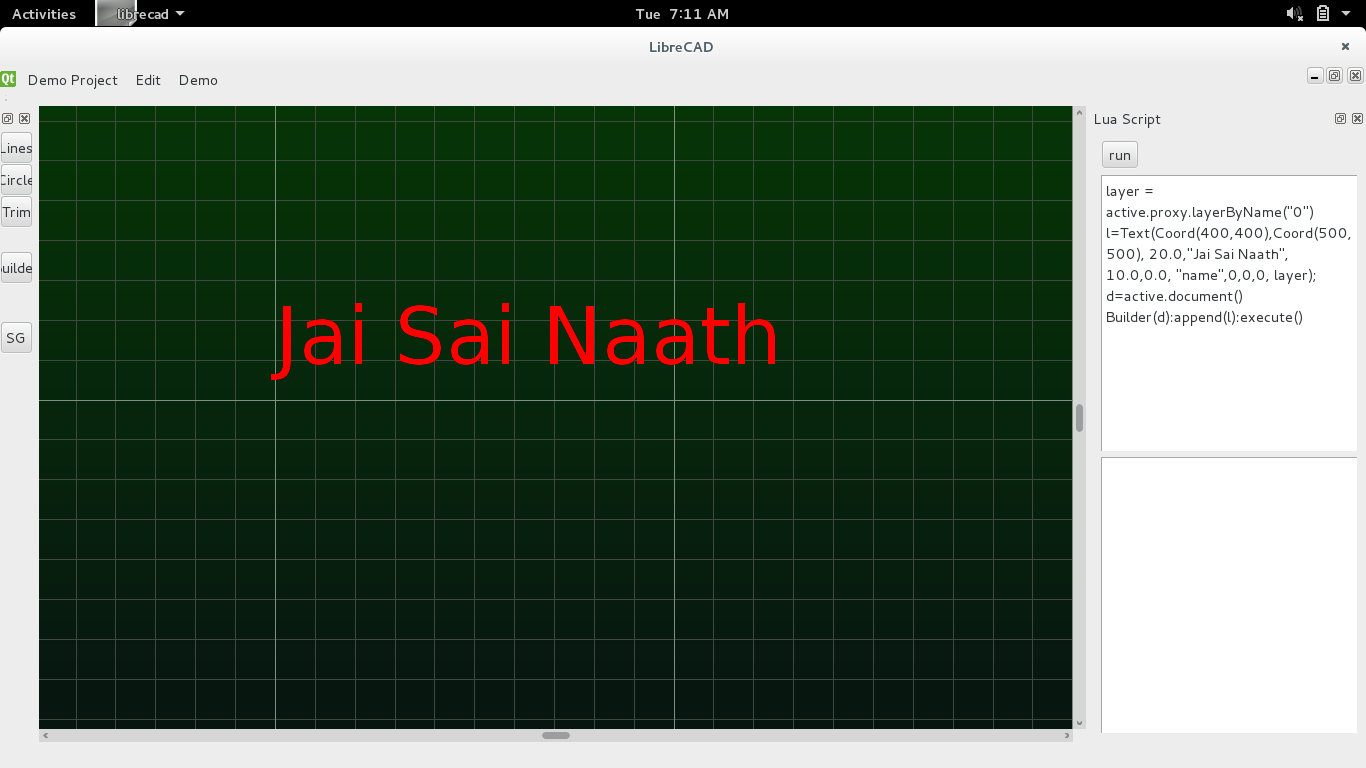
\includegraphics[scale=0.3]{images/cad/text.png}
\caption{ The Text entity implementation. }
\end{center}
\end{figure}
\begin{figure}[h]
\begin{center}
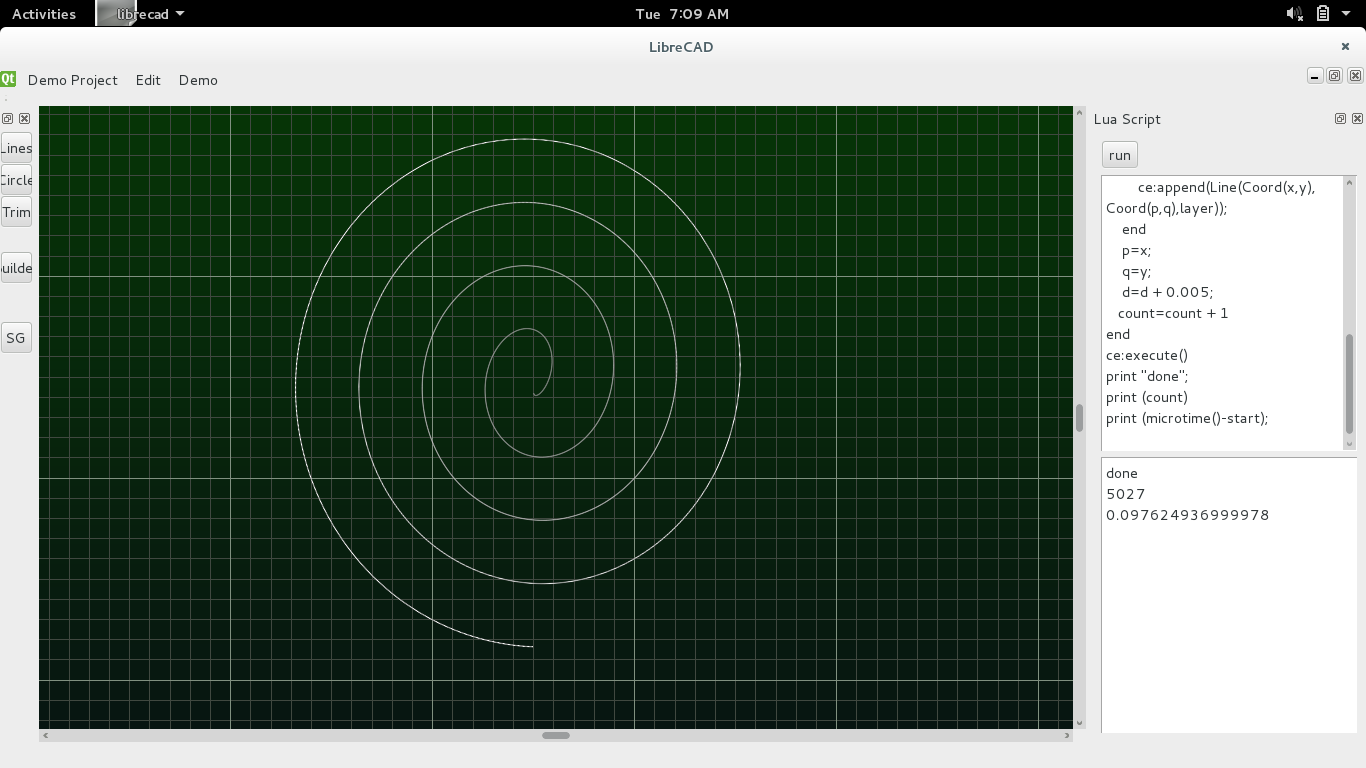
\includegraphics[scale=0.3]{images/cad/spiral.png}
\caption{ Spiral Drawn with the scripting module of LibreCAD 3 using Lua language. }
\end{center}
\end{figure}
\begin{figure}[h]
\begin{center}
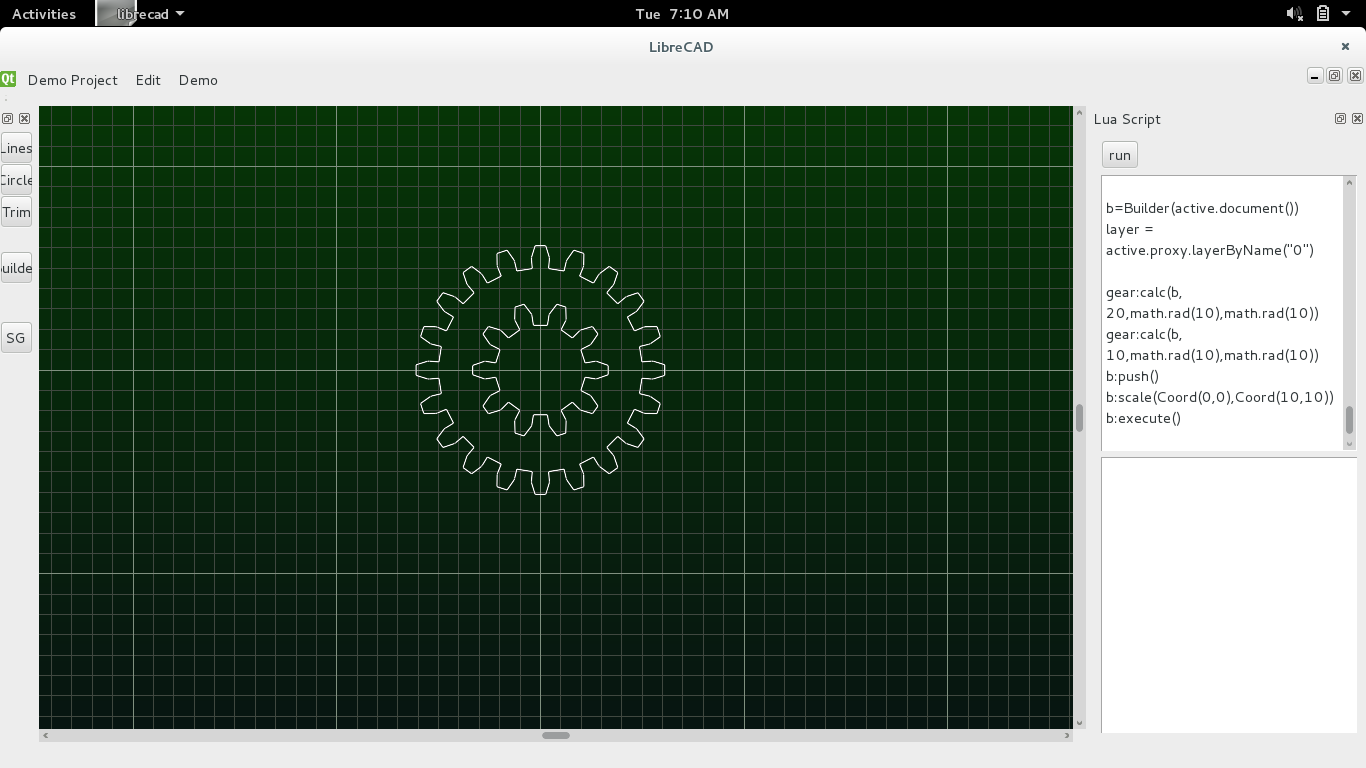
\includegraphics[scale=0.3]{images/cad/gear.png}
\caption{ Gear module drawn using LibreCAD 3 scripting.}
\end{center}
\end{figure}
\begin{figure}[h]
\begin{center}
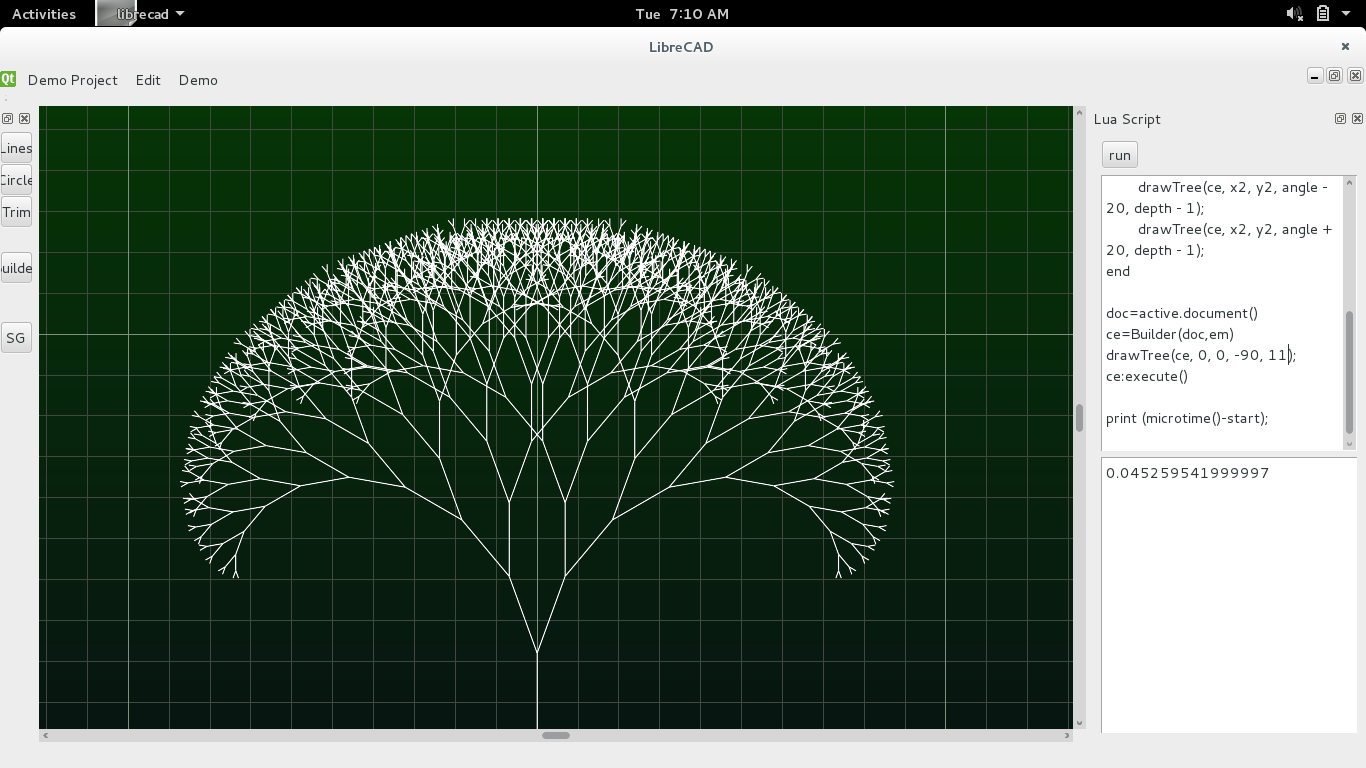
\includegraphics[scale=0.3]{images/cad/fractaltree.png}
\caption{ fractaltree drawn using LibreCAD 3 scripting. }
\end{center}
\end{figure}

\subsection{Installation Guide}
To install v3, you need to clone it from github.
\begin{itemize}
\item Go to terminal and type\\\\
\textit{git clone http://www.github.com/gaganjyot/LibreCAD3.git}
\item Now go to the directory vEdit by using: \\\\
\textit{cd LibreCAD3}
\item Now running cmake command: \\\\
\textit{cmake vEdit.pro}
\item Now MakeFile will be generated. After that run make: \\\\
\textit{make}
\item An executable file will be generated. Execute it using: \\\\
\textit{./lcUI/librecad}
\end{itemize}

\chapter{Technologies Used}
\input{input/qt.tex}
\newpage
\section{Introduction to \LaTeX}

\LaTeX, I had never heard about this term before doing this project,
but when I came to know about its features, found it excellent. 
\LaTeX{} (pronounced /ˈleɪtɛk/, /ˈleɪtɛx/, /ˈlɑːtɛx/, or /ˈlɑːtɛk/) is a 
document markup language and document preparation system for the \TeX{} 
typesetting  program. Within the typesetting system, its name is styled 
as \LaTeX.

\image{0.9}{images/donald.png}{Donald Knuth, Inventor Of \TeX{} 
typesetting system}

Within the typesetting system, its name is styled as \LaTeX. The term 
\LaTeX{} refers only to the language in which documents are written, 
not to the editor used to write those documents. In order to create a 
document in \LaTeX, a .tex file must be created using some form of text 
editor. While most text editors can be used to create a \LaTeX{} document, 
a number of editors have been created specifically for working with \LaTeX.

\LaTeX{} is most widely used by mathematicians, scientists, 
engineers, philosophers, linguists, economists and other scholars in 
academia. As a primary or intermediate format, e.g., translating DocBook 
and other XML-based formats to PDF, \LaTeX{} is used because of the 
high quality of typesetting achievable by \TeX. The typesetting system 
offers programmable desktop publishing features and extensive facilities 
for automating most aspects of typesetting and desktop publishing, 
including numbering and cross-referencing, tables and figures, 
page layout and bibliographies.

\LaTeX{} is intended to provide a high-level language that
accesses the power of \TeX. \LaTeX{} essentially comprises a
collection of \TeX{} macros and a program to process \LaTeX documents. 
Because the \TeX{} formatting commands are very low-level, it is usually 
much simpler for end-users to use \LaTeX{}.


\subsection{Typesetting}
\LaTeX{} is based on the idea that authors should be able to focus on 
the content of what they are writing without being distracted by its 
visual presentation. In preparing a \LaTeX{} document, the author 
specifies the logical structure using familiar concepts such as 
chapter, section, table, figure, etc., and lets the \LaTeX{} system 
worry about the presentation of these structures. It therefore 
encourages the separation of layout from content while still allowing 
manual typesetting adjustments where needed. 

\begin{verbatim}
\documentclass[12pt]{article}
\usepackage{amsmath}
\title{\LaTeX}
\date{}
\begin{document}
  \maketitle 
  \LaTeX{} is a document preparation system 
  for the \TeX{} typesetting program.
   \par 
   $E=mc^2$
\end{document}
\end{verbatim}
\image{0.3}{images/latexoutput.png}{\LaTeX{} output of above program.}

\subsection{Installing \LaTeX{} on System}
Installation of \LaTeX{} on personal system is quite easy. As i have used \LaTeX{} on Ubuntu 13.04 so i am discussing the installation steps for Ubuntu 13.04 here:
\begin{itemize}
\item Go to terminal and type\\\\
\textit{sudo apt-get install texlive-full}
\item Your Latex will be installed on your system and you can check for manual page by typing.\\\\
\textit{man latex}\\
in terminal which gives manual for latex command.\\
\item To do very next step now one should stick this to mind that the document which one is going to produce is written in any type of editor whether it may be your most common usable editor Gedit or you can use vim by installing first vim into your system using command.\\\\
\textit{sudo apt-get install vim}\\
\item After you have written your document it is to be embedded with some set of commands that Latex uses so as to give a structure to your document. Note that whenever you wish your document to be looked into some other style just change these set of commands.\\\\
\item When you have done all these things save your piece of code with .tex format say test.tex. Go to terminal and type\\\\
\textit{latex path of the file test.tex Or pdflatex path of the file test.tex\\ eg: pdflatex test.tex}\\
for producing pdf file simultaneously.\\
After compiling it type command\\\\
\textit{evince filename.pdf\\ eg: evince test.pdf}\\
To see output pdf file. 
\end{itemize}

\subsection{Graphical Editors for \LaTeX{}}
\LaTeX{} is not restricted to command line only there are so many graphical based editors available to be used. These GUi based editors provide an easy interface to user so as to do typesetting in an efficient manner. Some of them are listed below:
\begin{itemize}
\item {Texmaker}
\begin{figure}[ht]
\centering
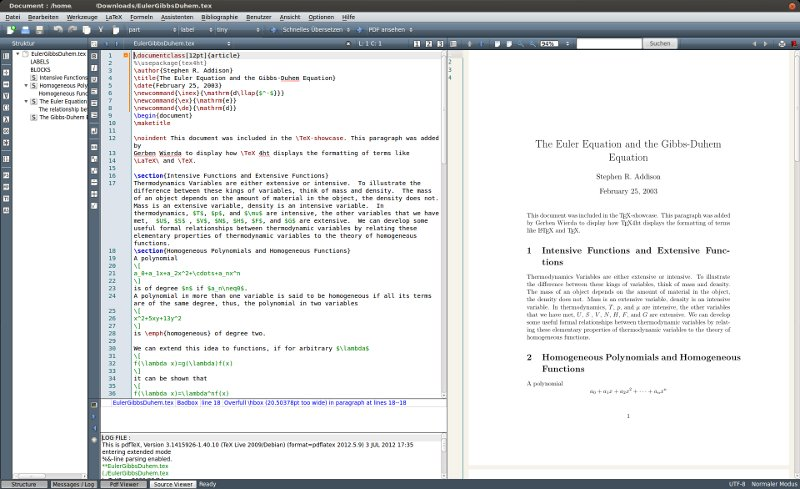
\includegraphics[scale=0.4]{images/texmaker.png}
\caption{Texmaker, A Graphical \LaTeX{} Editor}
\end{figure}
\item LEd
\begin{figure}[ht]
\centering
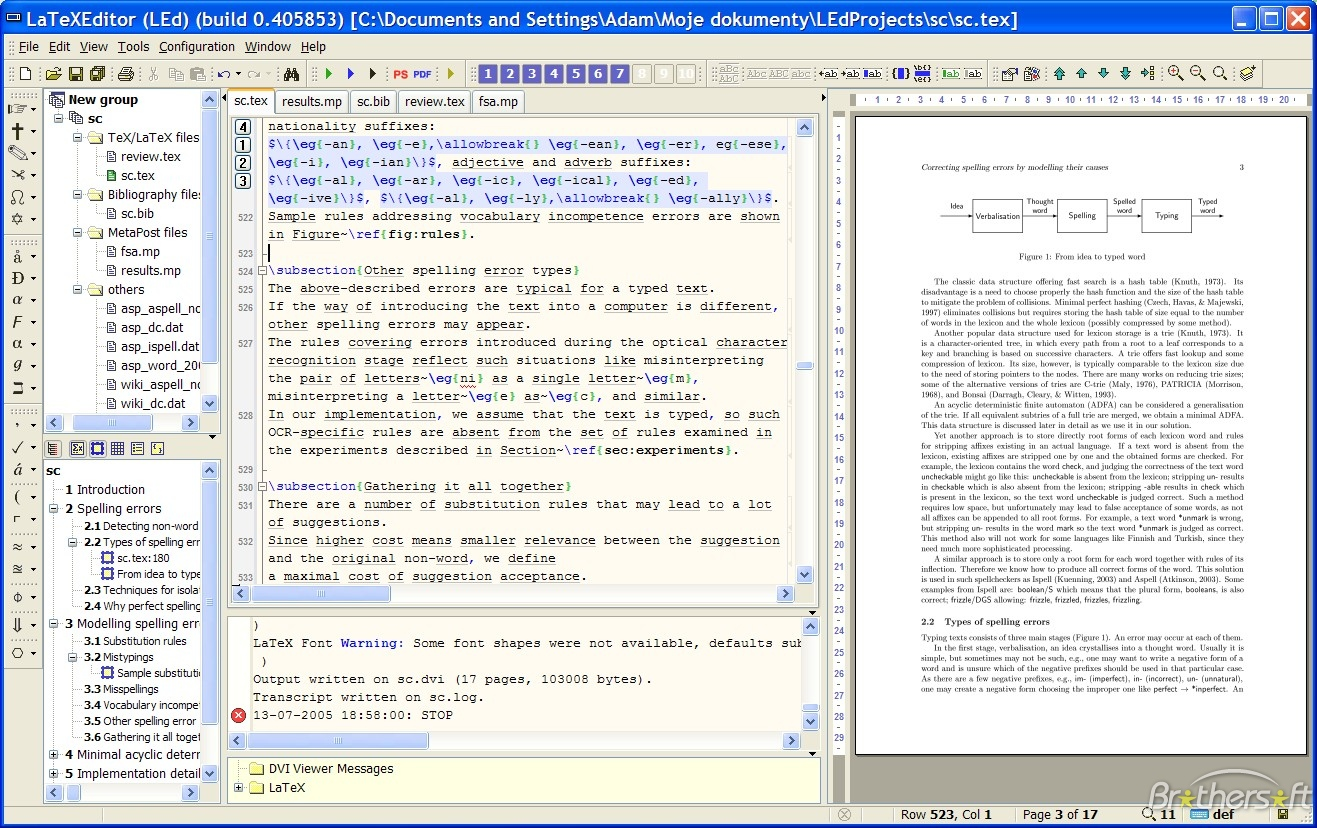
\includegraphics[scale=0.2]{images/led.png}
\caption{LEd, A Graphical \LaTeX{} Editor}
\end{figure}
\end{itemize}
And many more but the preferred method to produce \LaTeX{} document is through console mode only.


\subsection{Pdfscreen \LaTeX{}}
There are some packages that can help to have unified document using \LaTeX{}. Example of such a package is pdfscreen that let the user view it’s document in two forms-print and screen. Print for hard copy and screen for viewing your document on screen. Download this package from www.ctan.org/tex-archive/macros/latex/contrib/pdfscreen/.\\
Then install it using above mention method.\\
To test it the test code is given below:-\\
Just changing print to screen gives an entirely different view. But for working of pdfscreen another package required are comment and fancybox.\\\\
The fancybox package provides several different styles of boxes for framing and rotating content in your document. Fancybox provides commands that produce square-cornered boxes with single or double lines, boxes with shadows, and round-cornered boxes with normal or bold lines. You can box mathematics, floats, center, flushleft, and flushright, lists, and pages.\\\\
Whereas comments package selectively include/excludes portions of text. The comment package allows you to declare areas of a document to be included or excluded. One need to make these declarations in the preamble of your file. The package uses a method for exclusion that is pretty robust, and can cope with ill-formed bunches of text.\\\\
So these extra packages needed to be installed on system for the proper working of pdfscreen package.
\subsection{Web based graphic generation using \LaTeX{}}
\LaTeX{} is also useful when there is need of generating the graphics from browser. For
example to draw a circle by just entering its radius in html input box. So this kind
A
of project can be conveniently handled using \LaTeX{}. Basic idea behind this generation
process is that when user clicks on submit button after entering radius a script will run
that enter the radius in already made .tex file and recompiles it on server and makes its
pdf and postscript file. After that user can view those files by clicking on link provided
to view the files. See some screen shots of such a graphic generation project made by
Dr. H.S. Rai:\\
So here in the above input page which is also the index page user can enter input
for length of rectangle, breadth of rectangle and for radius of circle after that user can submit the values. After the values get submitted a script get runs by php code at server
side. This script first enters the dimensions of rectangle and circle that were selected by
user in to an already existing .tex file and replace with the older dimensions there. After
that script recompiles the the tex file and make it available for user.\\
In above figure it gets clear that .tex file has been compiled and pdf and postscript files
are available to user and user can download the graphics so produced. Hence graphics
can be generated in \LaTeX{} through web interface.
\begin{figure}[ht]
\centering
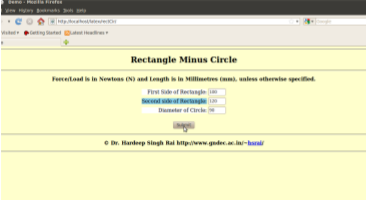
\includegraphics[scale=0.5]{images/webgraphic.png}
\caption{Web based graphic generation using \LaTeX{}(input page)}
\end{figure}

\input{input/cairo.tex}

\chapter{Project Legacy}
\input{input/legacy.tex}

\begin{thebibliography}{9}
\bibitem{} LibreCAD 3, https://github.com/gaganjyot/LibreCAD\_3
\bibitem{} My Blog, http://codebasement.wordpress.com
\bibitem{} My Github Profile, http://github.com/gaganjyot
\end{thebibliography}

\end{document}

